% Fig 3.20 57Fe nuclear levels under successive perturbations:
% isomer shift (both levels raised), quadrupole splitting of I=3/2,
% magnetic splitting (I=3/2 -> four, I=1/2 -> two sublevels) with the six
% allowed Delta m_I = 0,+/-1 absorption transitions.
\documentclass[tikz,border=5pt]{standalone}
\usetikzlibrary{arrows.meta}
\usepackage{amsmath}
\usepackage{bm}
\usepackage{fontspec}
\setmainfont{Times New Roman}
\begin{document}
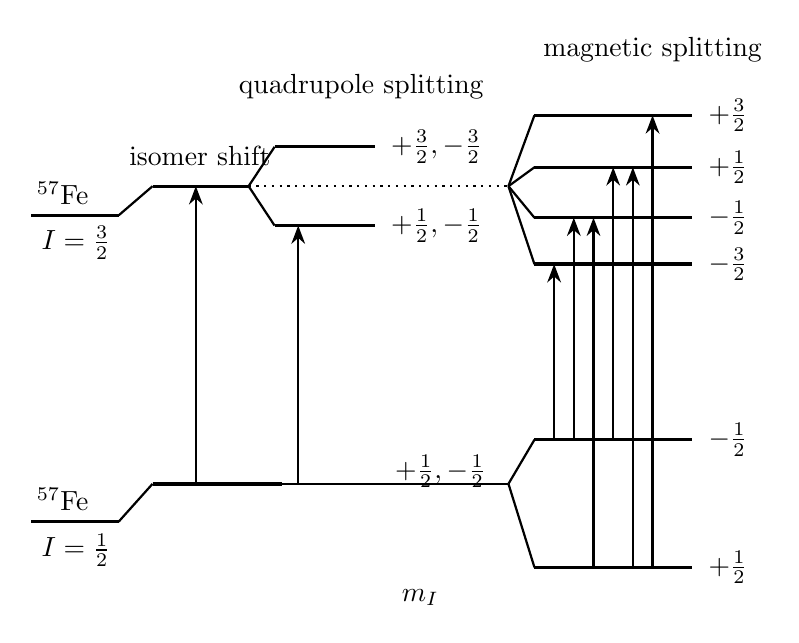
\begin{tikzpicture}[line width=0.8pt,>=Stealth]
% ---------- unperturbed levels ----------
\draw[very thick] (0.11,5.27) -- (1.22,5.27);
\node[anchor=west] at (0.05,5.55) {$^{57}$Fe};
\node[anchor=west] at (0.11,4.92) {$I=\tfrac{3}{2}$};
\draw[very thick] (0.11,1.38) -- (1.22,1.38);
\node[anchor=west] at (0.05,1.66) {$^{57}$Fe};
\node[anchor=west] at (0.11,1.02) {$I=\tfrac{1}{2}$};
% ---------- isomer shift ----------
\draw (1.22,5.27) -- (1.65,5.64);
\draw[very thick] (1.65,5.64) -- (2.87,5.64);
\draw (1.22,1.38) -- (1.65,1.86);
\draw[very thick] (1.65,1.86) -- (3.30,1.86);
\draw[->] (2.20,1.86) -- (2.20,5.64);
\node at (2.25,6.02) {isomer shift};
% ---------- quadrupole splitting (excited state only) ----------
\draw (2.87,5.64) -- (3.20,6.14);
\draw (2.87,5.64) -- (3.20,5.14);
\draw[dotted] (2.87,5.64) -- (6.17,5.64);
\draw[very thick] (3.20,6.14) -- (4.47,6.14);
\node[anchor=west] at (4.55,6.14) {$+\tfrac{3}{2},-\tfrac{3}{2}$};
\draw[very thick] (3.20,5.14) -- (4.47,5.14);
\node[anchor=west] at (4.55,5.14) {$+\tfrac{1}{2},-\tfrac{1}{2}$};
\draw[->] (3.50,1.86) -- (3.50,5.14);
\node at (4.30,6.90) {quadrupole splitting};
% ground state continues unsplit
\draw (3.30,1.86) -- (6.17,1.86);
\node[anchor=west] at (4.60,2.02) {$+\tfrac{1}{2},-\tfrac{1}{2}$};
% ---------- magnetic splitting ----------
\draw (6.17,5.64) -- (6.50,6.54);
\draw (6.17,5.64) -- (6.50,5.88);
\draw (6.17,5.64) -- (6.50,5.24);
\draw (6.17,5.64) -- (6.50,4.65);
\draw[very thick] (6.50,6.54) -- (8.50,6.54);
\node[anchor=west] at (8.58,6.54) {$+\tfrac{3}{2}$};
\draw[very thick] (6.50,5.88) -- (8.50,5.88);
\node[anchor=west] at (8.58,5.88) {$+\tfrac{1}{2}$};
\draw[very thick] (6.50,5.24) -- (8.50,5.24);
\node[anchor=west] at (8.58,5.24) {$-\tfrac{1}{2}$};
\draw[very thick] (6.50,4.65) -- (8.50,4.65);
\node[anchor=west] at (8.58,4.65) {$-\tfrac{3}{2}$};
\draw (6.17,1.86) -- (6.50,2.42);
\draw (6.17,1.86) -- (6.50,0.80);
\draw[very thick] (6.50,2.42) -- (8.50,2.42);
\node[anchor=west] at (8.58,2.42) {$-\tfrac{1}{2}$};
\draw[very thick] (6.50,0.80) -- (8.50,0.80);
\node[anchor=west] at (8.58,0.80) {$+\tfrac{1}{2}$};
\node at (8.00,7.38) {magnetic splitting};
% six allowed transitions
\draw[->] (6.75,2.42) -- (6.75,4.65);
\draw[->] (7.00,2.42) -- (7.00,5.24);
\draw[->] (7.25,0.80) -- (7.25,5.24);
\draw[->] (7.50,2.42) -- (7.50,5.88);
\draw[->] (7.75,0.80) -- (7.75,5.88);
\draw[->] (8.00,0.80) -- (8.00,6.54);
% magnetic quantum number label
\node at (5.05,0.42) {$m_I$};
\end{tikzpicture}
\end{document}
